%= local definitions of macros ============================
\newcommand{\Herwig}{H\protect\scalebox{0.8}{ERWIG}\xspace}
\newcommand{\Pythia}{P\protect\scalebox{0.8}{YTHIA}\xspace}
\newcommand{\Sherpa}{S\protect\scalebox{0.8}{HERPA}\xspace}
\newcommand{\Rivet}{R\protect\scalebox{0.8}{IVET}\xspace}
\newcommand{\Professor}{P\protect\scalebox{0.8}{ROFESSOR}\xspace}
\newcommand{\eps}{\varepsilon}
\newcommand{\mc}[1]{\mathcal{#1}}
\newcommand{\mr}[1]{\mathrm{#1}}
\newcommand{\mb}[1]{\mathbb{#1}}
\newcommand{\tm}[1]{\scalebox{0.95}{$#1$}}
\newcommand{\SMEFTsim}{\texttt{SMEFTsim}}
\newcommand{\SMEFTatNLO}{\texttt{SMEFT@NLO}}
\newcommand{\Madgraph}{M\protect\scalebox{0.8}{ADGRAPH}\xspace}
%= title + authors =====================================
\section{Study of EFT effects in loop induced Higgs processes ~\protect\footnote{
  A.~Cueto,
  S.~Pigazzini}{}}

%= MANDATORY label ======================================
\label{sec:projname}

%= (optional) preamble ================================== 
%\begin{abstract}

%\end{abstract}

%= content ===== ========================================
\subsection{Introduction}
\label{sec:higgseft:section1}
The Standard Model Effective Field Theory (SMEFT) approach is a powerful tool to look for hints of new physics. It allows to study large sets of experimental data without assuming that the theory used is valid to arbitrarily high energies. In the SMEFT, the Standard Model (SM) as we know it is just an effective theory at energies around the electroweak scale. Beyond the Standard Model (BSM) physics manifests at higher scales, $\Lambda$, and is parameterised in terms of higher-dimmensional operators that conserve the same fields and symmetries as the SM. At any mass dimension, a complete bases of non-reduntant operators can be worked out and the full Lagrangian can be written as a power expansion
\begin{equation}
\mathcal{L}_{\textrm SMEFT} = \mathcal{L}_{\textrm SM} + \sum_{d>4}\sum_{i}\frac{c_i}{\Lambda^{d-4}}\mathcal{O}_{i}^{(d}),
\end{equation}  

where $\mathcal{L}_{\textrm SM}$ is the SM Lagrangian, $c_i$ are the Wilson coefficients and ${\mathcal{O}^{d}}$ the set of independent operators for dimension $d$. Operators with $d=5,7$  violate lepton and/or baryon number conservation~\cite{Degrande:2012wf,Kobach:2016ami}. Thus, dimension-6 operators represent the leading deviation from the SM and will be the focus of this work. The modification of a cross section by the insertion of one dimesion-6 operator in the amplitudes can be written as

\begin{equation}
\sigma = \sigma_{\textrm SM} + \sum_{i}\sigma_i^{\textrm int} \frac{c_i}{\Lambda^{2}} + \sum_{i,j}\sigma_{(i,j)}^{\textrm BSM} \frac{c_ic_j}{\Lambda^{4}} ,
\end{equation}  

where $\sigma_{\textrm SM}$ is the SM cross section of a given process, $\sigma_i^{\textrm int}$ is the interference between the SM and the BSM amplitudes and $\sigma_{(i,j)}^{\textrm BSM}$ represents the pure BSM correction to the SM cross section. The leading term is formally $\sigma_i^{\textrm int}$ and the one than will be investigated in this work. 

Several bases of independent operators can be found in the literature~\cite{Grzadkowski:2010es,Contino:2013kra,Gupta:2014rxa,Masso:2014xra}. In the context of the study of the Higgs boson, the SILH basis~\cite{Contino:2013kra} has been commonly used. However, it is not optimised for, for example, diboson processes. Even if the translation between bases is known and has been automated~\cite{Falkowski:2015wza,Aebischer:2017ugx}, experimental collaboration have started to publish their EFT interpretations in the Warsaw basis also in the Higgs sector~\cite{ATLAS:2019jst,ATL-PHYS-PUB-2019-042} to facilitate future global fits of electroweak, Higgs and top data.

The procedure to test the EFT effects for a given set of measurements can be tedious in practice and a big effort has been devoted to develop public code to perform this task in a automatic and generic way~\cite{Brivio:2019irc}. For the Warsaw basis, different Universal FeynRules Output (UFO)~\cite{Degrande:2011ua} models are available which can be interfaced with modern event generators.

The \SMEFTsim\ code~\cite{Brivio:2017btx} is a well documented UFO implementation of the full set of dimension-6 operators in the Warsaw basis. Its main scope is the estimation of the leading SMEFT corrections to the SM. The effective Lagrangian is truncated at $\Lambda^{-2}$ and not supported for next-to-leading-order (NLO) simulations. For Higgs data interpretation the model have become of common use due to its completeness~\cite{Ellis:2018gqa,ATLAS:2019jst}.  To reproduce all the main Higgs production and decay channels in the SM, the loop-induced processes ($hgg$, $h\gamma\gamma$,$hZ\gamma$) are included as effective vertices. However, this implementation might not result satisfactory for reasons as the ones exposed below:
\begin{itemize}
\item Only operators with the same point-like structure as the effective vertices included to reproduce loop-induced processes can modify the cross sections of these processes. That means that, for example, a modification of the top Yukawa will not affect the gluoon-gluon fusion process.
\item Given the truncation of the Lagrangian, operators that enter in the shifts to input parameters and that will modify the cross section of any tree-level process does not modify the cross section of loop-induced processes.
\item A reliable computation of the Higgs plus jet  production in gluon-gluon fusion requires top quark loop amplitudes at high $p_{\textrm T}$ and the implementation of $gggH$ vertices.
\item The $gg\to ZH$ process cannot be simulated.
\end{itemize}

To overcome these concerns the \SMEFTatNLO\ tool~\cite{SMEFTNLO} can be used for the loop induced Higgs processes. The tool includes a complete implemation of the SMEFT compatible with NLO QCD predictions. In this work, we study the $gg\to ZH$ and $gg\to H$ processes using this tool. 







\subsection{Comparison between models}
\label{sec:higgseft:section2}
The \SMEFTsim and \SMEFTatNLO tools have been validated against each other~\cite{Durieux:2019lnv}. In this section we compare both models at leading order (LO) by checking the cross sections of the $pp\to ZH$ and $pp\to t\bar{t}H$ processes. The comparison is made at the cross section level and, thus, not expected to be in perfect agreement since it will be affected by phase-space integration. The main goal of this comparison is to show the mapping between the different Wilson coefficients naming and to ensure that the setup used for both models is consistent.

For both models we use the $m_Z$, $m_W$, $G_F$ scheme of electroweak parameters\footnote{We use the \texttt{SMEFTsim\_A\_U35\_MwScheme\_UFO} model for \SMEFTsim and the \texttt{SMEFTatNLO\_U2\_2\_U3\_3\_cG\_4F\_LO\_UFO-LO} model for \SMEFTatNLO}. The \Madgraph 2.6.6 generator is used to obtain the cross sections results. The definition of the processes is as follows for the SM results:

\noindent
{\bf ttH:}\\
\noindent
  \texttt{ define p = p b b$\sim$ }\\
  \texttt{ generate p p $>$ h t t$\sim$ SMHLOOP=0 NP=0 }

\noindent
{\bf ZH:}\\
  \noindent
  \texttt{ define p = p b b$\sim$} \\
  \texttt{ generate p p $>$ h l+ l- SMHLOOP=0  NP=0     }\\
  
  The values of several parameters like $m_W$, $mt$, $\alpha_S$ or $\Gamma H$ differ in the default settings of the models and they were set to the same values.

  The tables below show the comparison between the predictions obtained for SM in both models as well as the interference terms, obtained with the NP$^{\wedge}$2$==$1 (NP$^{\
\wedge}$2$==$2)  for the SMEFTsim (SMEFTatNLO) model, of the SM and the BSM turning all Wilson coefficients to 0.0 except the one we are testing.\\

\begin{table}[h]
\begin{tabular}{|l|c|c|}
\hline
\textbf{Operator} & \textbf{SMEFTsim} & \textbf{SMEFTatNLO} \\
 \hline
 SM-SM & 0.25090E-01$\pm$ 0.98586E-04& 0.25474E-01$\pm$ 0.27461E-03\\
  \hline
cHbox-cpd & 0.30422E-02$\pm$ 0.11954E-04& 0.30887E-02 $\pm$ 0.33295E-04\\
 \hline
cHDD-cpDC & 0.41021E-03$\pm$ 0.14235E-04& 0.43339E-03$\pm$ 0.62340E-04\\
\hline
cHB-cpBB & 0.23066E-02$\pm$ 0.13620E-04& 0.22937E-02$\pm$ 0.40374E-04\\
 \hline
cHW-cpW & 0.18183E-01$\pm$ 0.71875E-04& 0.18365E-01$\pm$ 0.19500E-03\\
 \hline
cHWB-cpWB & 0.83775E-02$\pm$ 0.37750E-04& 0.84396E-02$\pm$ 0.82850E-04\\
 \hline
cHd-cpd &-0.44477E-02$\pm$ 0.15107E-04&-0.44436E-02$\pm$ 0.43813E-04\\
 \hline
cHq3-c3pqi & 0.48815E-01$\pm$ 0.11144E-03& 0.47772E-01$\pm$ 0.49730E-03\\
\hline
cHe-cpe &-0.28531E-02$\pm$ 0.67446E-05& -0.14243E-02$\pm$ 0.13393E-04\\
cHe-cpmu & -0.28531E-02$\pm$ 0.67446E-05& -0.14243E-02$\pm$ 0.13393E-04\\
 \hline
cHl1-cpl1 & 0.32460E-02$\pm$ 0.15109E-04& 0.16375E-02$\pm$ 0.16110E-04\\
cHl1-cpl2 & 0.32460E-02$\pm$ 0.15109E-04& 0.16375E-02$\pm$ 0.16110E-04\\
\hline
cHl3-c3pl1 & -0.58824E-02$\pm$ 0.16581E-04& -0.36463E-02$\pm$ 0.49826E-04\\
cHl3-c3pl2 & -0.58824E-02$\pm$ 0.16581E-04& -0.36463E-02$\pm$ 0.49826E-04\\
\hline
\end{tabular}
\caption{ Comparison of the SM and interference predicitions for the Z($l^{+}l^{-}$)H process between the SMEFTsim and SMEFTatNLO}

\end{table}


\begin{table}[h]
\begin{tabular}{|l|c|c|}
\hline
\textbf{Operator} & \textbf{SMEFTsim} & \textbf{SMEFTatNLO} \\
 \hline
 SM-SM & 0.40168E+00$\pm$ 0.10096E-02& 0.40212E+00$\pm$ 0.25007E-02\\
 \hline
 cHbox-cpd & 0.48703E-01$\pm$ 0.12241E-03& 0.48756E-01$\pm$ 0.15501E-05\\
 \hline
 cHDD-cpDC & -0.12180E-01$\pm$ 0.24504E-04& -0.12223E-01$\pm$ 0.76085E-04\\
 \hline
 cHB-cpBB & 0.89346E-04$\pm$ 0.26491E-06& 0.89687E-04$\pm$ 0.82604E-06\\
 \hline
 cHW-cpW & 0.41603E-03$\pm$ 0.10884E-05& 0.42297E-03$\pm$ 0.40793E-05\\
 \hline
 cHWB-cpWB & -0.24990E-03$\pm$ 0.50055E-06& -0.25287E-03$\pm$ 0.16357E-05\\
 \hline
 cHd-cpd & -0.76148E-04$\pm$ 0.31512E-06& -0.76323E-04$\pm$ 0.15501E-05\\
 \hline
 cHq3-c3pqi & 0.20976E-02$\pm$ 0.56257E-05& 0.12428E-02$\pm$ 0.17784E-04\\
 \hline
 cuHAbs-ctp & -0.48847E-01$\pm$ 0.11970E-03& -0.49460E-01$\pm$ 0.30701E-03\\
 \hline
 cuGAbs-ctG & -0.33928E+00$\pm$ 0.87096E-03& 0.40722E+00 $\pm$ 0.24562E-02\\
 \hline
 cuBAbs-ctB & -0.82828E-03$\pm$ 0.20643E-05& 0.84754E-03$\pm$ 0.10257E-04\\
 \hline
 cuWAbs-ctW & -0.22186E-02$\pm$ 0.63027E-05& 0.22314E-02$\pm$ 0.22095E-04\\
  \hline
 cHl3-c3pl1 & -0.48889E-01$\pm$ 0.10230E-03& -0.24551E-01$\pm$ 0.15254E-03\\
 cHl3-c3pl2 & -0.48889E-01$\pm$ 0.10230E-03& -0.24551E-01$\pm$ 0.15254E-03\\
 \hline
  \end{tabular}
\caption{ Comparison of the SM and interference predicitions for the ttH process between the SMEFTsim and SMEFTatNLO}
\end{table}



\subsection{Kinematic studies for Higgs production in gluon-gluon fusion}
\label{sec:higgseft:section3}


\subsection{Simplified template cross section parametrization}
\label{sec:higgseft:section3}







To cite a paper, use bibtex:

Examples: Les Houches 2015 report~\cite{Badger:2016bpw},
paper~\cite{Aaboud:2016ffv}, tHV~\cite{'tHooft:1972fi}, and again~\cite{'tHooft:1972fi}

%See how nice it is if you use bibtex :)
Please remember to put the paper in the local bib file in the project
directory, see projname.bib. Someone will take care of processing this
file for the main document if it's not done automatically, but the
file needs to be a standard bib file, compliant with the rules...!

~\newline~
To reference and create labels within your contribution, use the conventions

fig:SM\_projname:figname

eq:SM\_projname:eqname

sec:SM\_projname:secname\\
Examples:
\begin{itemize}
\item Equation:
  \begin{equation}
    E = m c^2
    \label{eq:projname:eqemc2}
  \end{equation}
  Eq.~(\ref{eq:projname:eqemc2}) is very nice, and it is included in Sec.~\ref{sec:projname:section1}.
\item Figure: In Fig.~\ref{fig:projname:plot1} there's a plot:
\begin{figure}[htbp]
  \begin{center}
    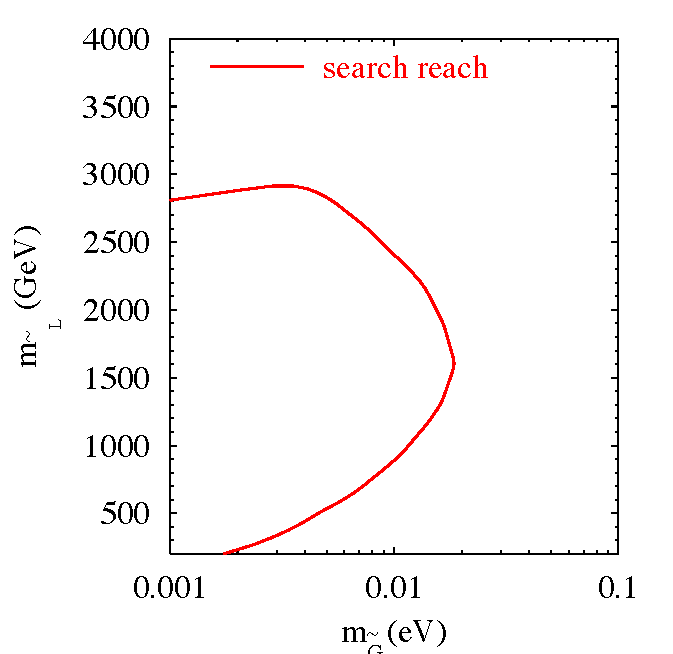
\includegraphics[width=5cm]{Fig1.pdf}
    \caption{...caption...}
    \label{fig:projname:plot1}
  \end{center}
\end{figure}
%% ~\newline~
%% To reference the main parts of the documents, use standard latex commands, with a prefix sec: and cha:.
%%
%% Examples: cha:nnlo will point to Chapter~\ref{cha:nnlo}.
%% Most likely, the conveners will fix these references at the end.
\end{itemize}
~\newline~
To use macros, define them locally, but then un-define them at the end of your local tex file.

Examples `` \Herwig{} `` is written using a macro, which is defined
in the local tex file, and undefined at the end of it.

\subsection{you can write subsections...}
Example of citation: in Ref.~\cite{Belanger:2014vza}

\subsubsection{and subsubsections...}

%= undefine macros (MANDATORY) ====================
\let\Herwig\undefined
\let\Pythia\undefined
\let\Sherpa\undefined
\let\Rivet\undefined
\let\Professor\undefined
\let\eps\undefined
\let\mc\undefined
\let\mr\undefined
\let\mb\undefined
\let\tm\undefined




